\documentclass[UTF8]{ctexart}
\usepackage{amsmath}
\usepackage{forest}
\usepackage{algorithm}
\usepackage{algorithmic}
\usepackage{graphicx}
\usepackage{tabularx}
\title{\vspace{-4cm}2023数据库概论第一次作业}
\author{2000013058 杨仕博}
\date{\today}
\begin{document}
\maketitle

\subsection{}

熵:熵是一个指标,他用来度量随机变量的混乱程度、系统的
混乱程度或者信息量的大小,对于
一个离散型随机变量$X$,其定义为
$H(X) = -\sum_{i=1}^{n}p_i\log p_i$,其中
$p_i$是$X$取第i个值的概率,n是一共可能的取值数目。

条件熵:条件熵是衡量在给定某事件发生的条件下衡量
另一个事件的不确定性的指标。离散型随机变量$X$关于
离散型随机变量$Y$的条件熵是
\[
\begin{aligned}
    H(X | Y) &= \sum\limits_{j = 1}^m p_j H(X | Y = y_j)\\
             &= -\sum\limits_{j = 1}^m p_j \sum\limits_{i = 1}^n p_{ij}\log p_{ij}
\end{aligned}
\]
其中,$p_j$是$Y$取到第j个值$y_j$的概率,
$p_{ij}$是$Y$取到$y_j$时$X$取到第i个值的概率

交叉熵:交叉熵是用来衡量两个概率分布差异性的指标,
对于两个概率分布$p, q$,若视$p$为基准的分布,则p和q的交叉熵
$H(p, q) = \sum\limits_{i = 1}^np(x_i)\log(\frac{1}{q(x_i)})$,
其中两个分布一共有n种可能取值,$x_1, ..., x_n$,$p(x_i), q(x_i)$
是其概率。

相对熵是衡量两个概率分布的差异的非对称性度量。对于分布
$p, q$,其相对熵为
$KL(p || q) = \sum\limits_{i = 1}^np(x_i)\log(\frac{p(x_i)}{q(x_i)})$,
其中变量的定义和上述交叉熵相同

\subsection{}

数据的独立性是指当数据结构发生变化时,我们通过系统提供的映
象(转换)功能,使应用程序不必改变,包含物理独立性和逻辑独
立性等。

数据库通过一下这些举措提高数据的独立性:

1. 把数据库定义和描述从应用程序中分离出去。

2. 对数据进行分级描述(全局逻辑、局部逻辑、存储)。

3. 数据存取由系统管理,用户不必考虑存取路。
径等细节,从而简化了应用程序(SQL)

\subsection{}

1. 数据定义独立性:文件系统数据与程序紧密结合、数据分散管理、
数据的语义信息只能由程序来解释且数据共享困难;而数据库系统
维护了面向全组织的数据结构,其数据反映了客观事物间的本质联系,
且记录之间无联系。

2. 数据完整性独立性:文件系统的数据存在很多副本,给数据的修
改与维护带来了困难,容易造成数据的不一致性;而数据库中的数据
面向整个系统,而不是面向某一应用,数据集中管理,数据共享,
每个应用选用数据库的一个子集,只要重新选取不同子集或者加上一
小部分数据,就可以满足新的应用要求。

3. 数据操作独立性:文件系统中的数据是字符流,数据查询困难,
每个查询都需要用户自己编程实现,而且需要重新编码;而数据库系统
把数据库定义和描述从应用程序中分离出去,使用分级的数据描述,
数据存取由系统管理,用户不必考虑存取路径等细节,从而简化了应
用程序。

4. 安全性:文件系统通常只提供基本的文件级别的权限控制;
而数据库提供了更好的安全性保障,提供了更复杂的访问
控制和加密认证特性。

\subsection{}

1. 对小型数据的存储:使用数据库可能过于复杂。

2. 大型二进制文件存储:对于较大的图像、音频和视频,使用数据
库可能增加不必要的复杂性。

\subsection{}

\begin{tabularx}{\linewidth}{|X|X|X|X|X|}
\hline
模型类型 & 模型结构 & 表达能力 & 数据独立性 & 操作简便性\\
\hline
层次模型    
& 树状结构 
& 支持的联系种类太少 
& 数据独立性较强,在多个表中分布的数据易于维护和修改 
& 操作简单\\
\hline
网状模型    
& 网络结构 
& 表达的联系种类丰富 
& 数据依赖关系复杂,难以维护和修改 
& 操作繁琐\\
\hline
关系模型    
& 用二维表来表示实体及其相互联系 
& 适合刻画实体间的关系和属性,具有良好的表达能力 
& 数据独立性高:用户只需提出“做什么”,无须说明“怎么做” 
& 操作简单,易于理解和查询\\
\hline
面向对象模型 
& 基于面向对象的编程思想,将数据和操作封装为对象 
& 适合表达实体的属性、关系和操作,具有强大的表达能力 
& 数据独立性较强,支持继承和多态,易于维护和修改 
& 操作相对复杂,需要掌握面向对象编程思想和语言特性\\
\hline
\end{tabularx}

\subsection{}

1. 科学计算领域,往往需要高效存储和操作多维数据。

2. 业务分析领域,往往需要对大量数据进行分析和统计,多维数组
可以方便地存储和处理这些数据,并支持复杂的数据查询和分析。

\subsection{}

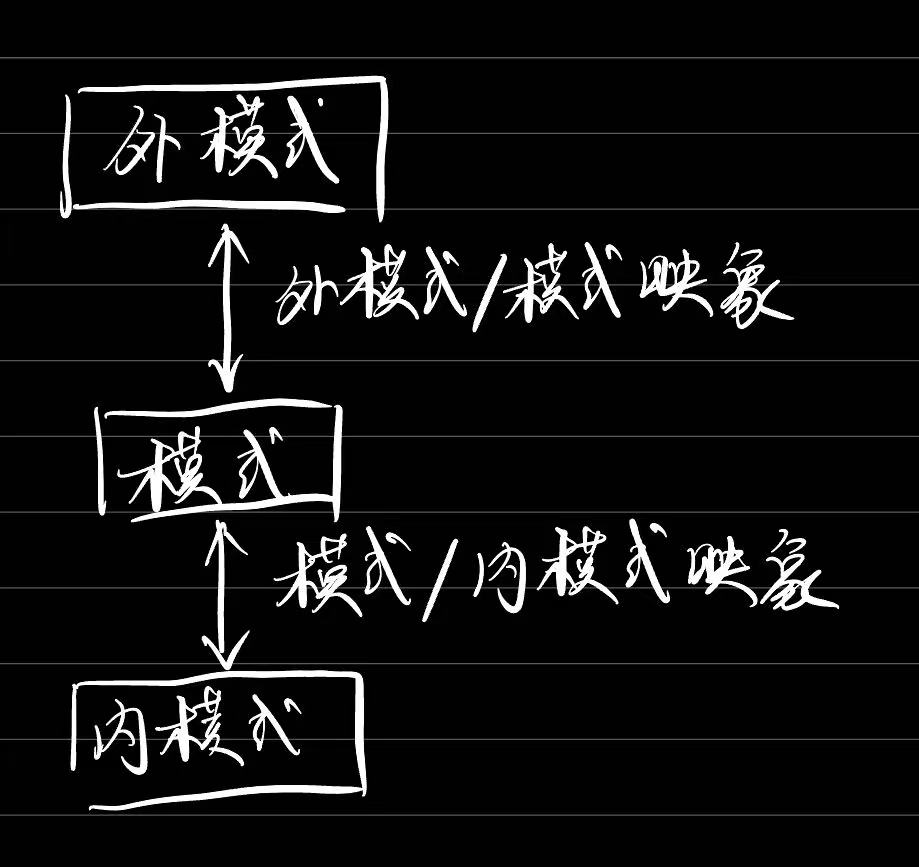
\includegraphics[width=.8\textwidth]{./pics/1.jpeg}

好处:

1. 数据独立性:通过两层映像保证模式/存储结构更改时,外模式
/模式保持不变,从而应用程序可以保持不变,以达成数据的逻辑/物理
独立性。

2. 数据安全性:通过多层分层使得用户无法直接访问模式层,从而保
障了数据安全。

3. 数据共享性:模式层可以为多个应用程序提供统一的数据访问接口,
从而实现数据共享,避免了数据的冗余和数据不一致的问题。

4. 系统维护性:分层结构使得维护系统更加方便了,数据库备份和恢复
时不需要备份和恢复应用程序和模式层的相关信息。

\subsection{}

1. 查询方式上,搜索引擎的关键字查询基于全文检索进行,而数据库
需要根据数据模型和数据结构编写相应的针对某些特定内容(如属性)
的查询语句。

2. 查询结果中,前者返回有序文档列表,后者返回符合条件的一组数
据记录。

3. 查询精度上,搜索引擎的搜索结果中可能存在垃圾信息或不相关的
信息,而数据库查询上精确的查询条件匹配。

4. 数据处理能力上,搜索引擎可以处理大量非结构数据,而数据库主要
用于处理结构化数据。

5. 查询效率上,搜索引擎需要扫描大量文档和索引,相对较慢,而数据
库查询则可以通过索引优化查询语句以得到更高的效率。

\subsection{}

(1)

1. 数据库运行管理:并发控制、存取控制、完整性约束条件检查和
执行,日志组织和管理,事务管理和自动恢复

2. 数据组织存储和管理:用户数据、索引、数据字典的组
织、存储和管理,包括文件结构、存取方式、数据之间联系的实现

3. 数据库建立和维护功能:数据的装入、转换、卸出:数据库
的转储、恢复、性能监视和分析

(2)

他并不需要复杂的数据库运行管理,如并罚控制、事物管理等,也不需要
复杂的用于数据库维护的功能,比如性能监视和分析。

\subsection{}

职能:

在建库方面,他需要负责确定模式、外模式、存储结构以及存取策略;
负责数据的整理和装入。

在用库方面,他需要定义完整性约束条件,规定数据的保密级别、用户
权限;监督和控制数据库的运行情况;制定后援和恢复策略,负责故障
恢复。

在改进方面,他需要监督分析系统的性能(空间利用率,处理效率),进
行数据库重组织,物理上重组织,以提高性能;进行数据库重构造,设计上较大
改动,模式和内模式修改

技能:

技术上,需要擅长使用数据应用,能够保障数据安全;组织上,需要
擅长处理数据生命周期的问题和置顶数据战略;制度上,需要擅长数据
治理和数据架构的搭建;流程上,需要擅长控制数据质量和制定与保障
数据标准。

\subsection{}

1.Workload 预测

2.智能调参

3.异常检测(预测)

4.冷热分离

5.智能调度与负载均衡

6. Learned Index/LRU 等数据结构

7.SQL 优化器建模

8. 数据库系统

(来源:https://www.zhihu.com/question/312350519/answer/1444423751)

\end{document}